\chapter{Simulación y optimización}
\label{cap:simulacion}

\section{Configuración de las instancias empleadas para la simulación del tráfico}

\subsection{Instancias sin semáforos}

Actualmente, la rotonda de Padre Anchieta no cuenta con ningún semáforo. La regulación del tráfico se produce únicamente por dos factores: la señalización (señales de ceda el paso, principalmente) y los pasos de peatones, los cuales hemos tenido en cuenta a la hora de evaluar el comportamiento del tráfico.

Asimismo, la simulación de estas instancias realizaría una función de control con respecto a las instancias con semáforos, puesto que nos permitiría comparar el rendimiento de la rotonda actual con el caso de que tuviera semáforos.

Se proponen tres instancias:

\paragraph{\texttt{anchieta\_no\_tls.}}

Es la instancia más sencilla, puesto que únicamente se simulará tráfico rodado sin tener en cuenta a los peatones.


\paragraph{\texttt{anchieta\_no\_tls\_few\_pedestrians.}}

Esta instancia es exactamente igual a la anterior, pero cuenta con aproximadamente 500 peatones generados con \texttt{randomTrips.py} mencionada en la sección~\ref{enfoque_estocastico}.


\paragraph{\texttt{anchieta\_no\_tls\_many\_pedestrians.}}

De nuevo, esta instancia es idéntica a las dos primeras, con la salvedad de que cuenta con aproximadamente 2000 peatones generados con la misma herramienta, \texttt{randomTrips.py}.


Tal y como se mencionó en la sección~\ref{enfoque_estocastico}, la generación de los peatones es completamente aleatoria y distribuida uniformemente tanto en tiempo (una hora de simulación) como en espacio, puesto que desafortunadamente no existen datos lo suficientemente granulares sobre los movimientos de los peatones en la zona.


\subsection{Instancias con semáforos}
\label{subsec:instancias}

Definidas las instancias anteriores, llega el momento de tomar una decisión importante: ¿dónde han de situarse los semáforos? A fin de cuentas, la rotonda de Padre Anchieta no es una zona que contara previamente con semáforos, por lo que nos corresponde a nosotros determinar la localización de estos.

Así pues, se proponen tres instancias con configuraciones semafóricas distintas:

\paragraph{\texttt{anchieta\_tls\_interior\_lane\_always\_green.}} Semáforos en cada entrada y salida, con el carril interior siempre en verde. Una posible configuración de los semáforos es añadir uno en cada entrada y salida de la rotonda, de modo que esté absolutamente regulada por estos. Además, el carril interior permanecería en verde siempre que fuera posible, cambiando de color únicamente en los casos en los que la vía entrada a la rotonda tenga dos carriles y sea necesario regular el paso entre los carriles izquierdos de la entrada y la rotonda. Esta instancia no necesita simular ningún peatón, puesto que todas las entradas y salidas estarían reguladas por semáforos y, por extensión, también los pasos de peatones. Ello hace innecesario evaluar cómo se comportarían los peatones durante la simulación (simplemente se quedarían parados mientras el semáforo peatonal cambia a verde para que puedan cruzar).

\paragraph{\texttt{anchieta\_tls\_interior\_lane\_changes.}} Semáforos en cada entrada y salida, con el carril interior cambiando de color. Es la misma configuración que la 1, con la salvedad de que el carril interior cambia de color junto con el exterior independientemente de que la entrada que se esté regulando tenga un carril o dos. El objetivo de simular estas dos configuraciones es comprobar cuál es más eficiente gestionando el carril interior. Véase la figura~\ref{fig:conf2}. Tanto en esta configuración como en la anterior, las fases se modificaron manualmente para garantizar que siguen un ciclo correcto. Esta instancia tampoco tiene en cuenta los peatones por los mismos motivos que la anterior.

\paragraph{\texttt{anchieta\_tls\_special\_few\_pedestrians.}} Semáforos al norte y al sur de la rotonda con pocos peatones. Este caso particular solamente instala dos semáforos: uno al norte de la rotonda (entre la entrada de la TF-5 en sentido Santa Cruz y la salida hacia la TF-5 en sentido La Orotava) y otro al sur (entre la salida hacia la TF-5 en sentido Santa Cruz y la entrada de doble carril desde la TF-5 en sentido La Orotava). Véase la figura~\ref{fig:conf3}. Esta instancia, dado que cuenta con pasos de peatones sin regular por semáforos, sí tendrá en cuenta durante la simulación a los peatones, cuya cantidad y rutas han sido definidas aleatoriamente por \texttt{randomTrips.py} dado que no existen datos medidos sobre tránsito de peatones en la zona. Esta instancia cuenta, aproximadamente, con 500 peatones.

\paragraph{\texttt{anchieta\_tls\_special\_many\_pedestrians.}} Semáforos al norte y al sur de la rotonda con muchos peatones. Esta instancia es idéntica a la anterior, con la salvedad de que se ha cuadruplicado la cantidad de peatones que circulan por la zona, para poder evaluar la circulación de los vehículos con un tránsito más denso de peatones.


\begin{figure}[ht]
    \centering
    \begin{subfigure}[t]{0.48\textwidth}
        \centering
        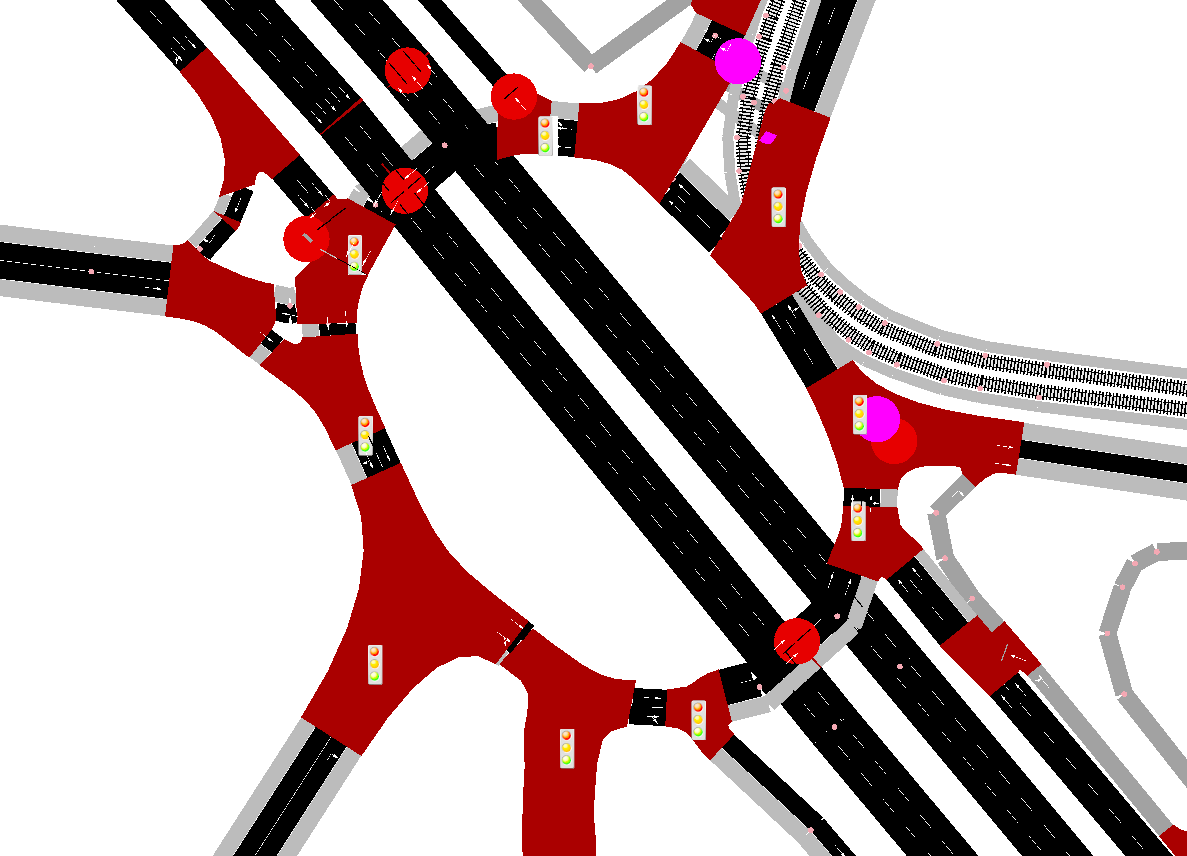
\includegraphics[width=\textwidth]{report/images/conf2.png}
        \caption{Imagen del archivo de red con los semáforos de las configuraciones 1 y 2.}
        \label{fig:conf2}
    \end{subfigure}
    \hfill
    \begin{subfigure}[t]{0.48\textwidth}
        \centering
        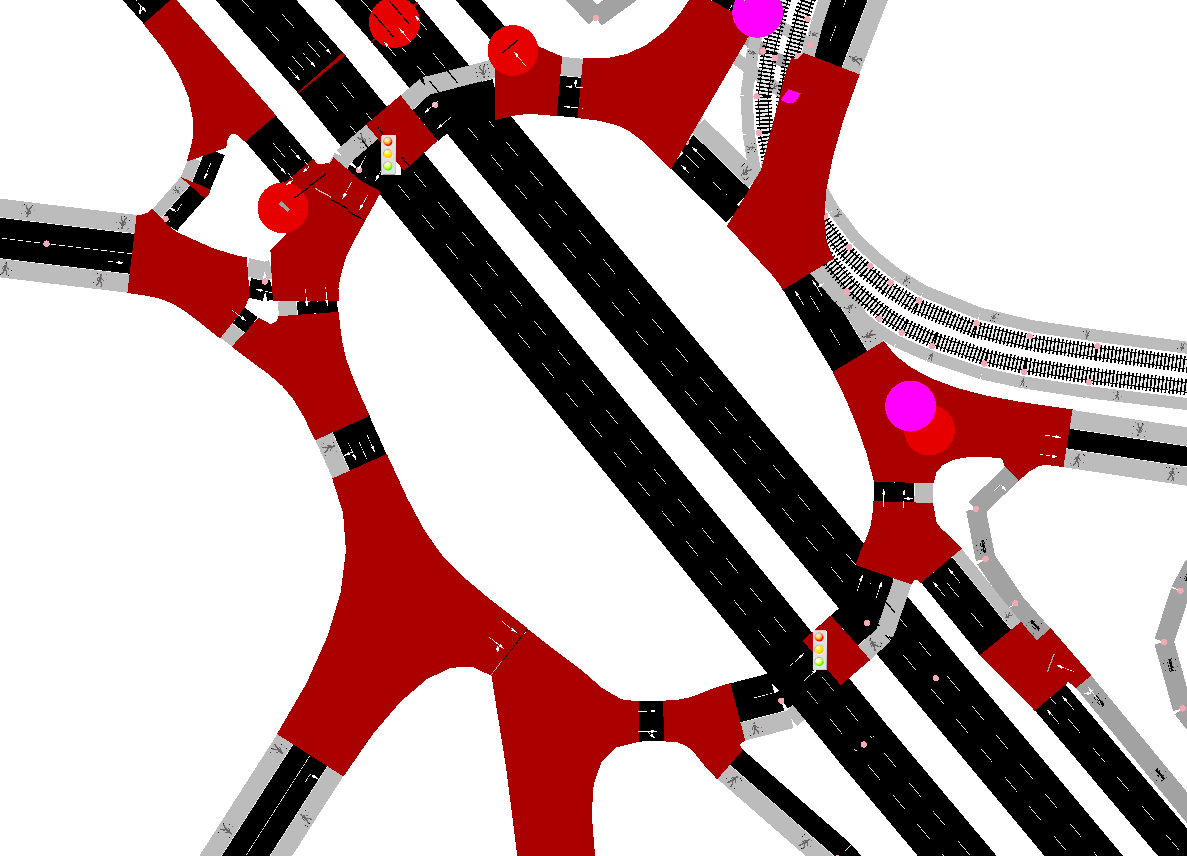
\includegraphics[width=\textwidth]{report/images/conf3.png}
        \caption{Imagen del archivo de red con los semáforos de la configuración 3 y 4.}
        \label{fig:conf3}
    \end{subfigure}
    \caption{Distintas configuraciones de los semáforos.}
    \label{fig:confs}
\end{figure}



\section{El algoritmo evolutivo}

Una vez se han definido los archivos de la simulación, corresponde evaluar la manera en que se va a implementar el algoritmo evolutivo. Para esto se ha empleado \texttt{Genetics.js}, una librería programada en TypeScript orientada a algoritmos evolutivos; en particular, algoritmos genéticos. Esta librería la programó Cristian Abrante, un antiguo alumno de la Escuela Superior de Ingeniería y Tecnología, para su TFG titulado <<Framework web de computación evolutiva>>~\cite{abrante_dorta_framework_2019}. 

Antes de proceder a emplear la librería, se hizo un fork de la misma y se realizaron algunos cambios. Los principales cambios están relacionados con la importación de módulos en TypeScript, de modo que todas las clases y elementos necesarios se pudieran importar directamente desde \texttt{genetics-js}. Asimismo, se modificó la librería para que los valores que el generador de números aleatorios que emplea el algoritmo pudiera detectar para qué fase en concreto estaba generando el valor, de modo que si cualquier fase contenía un semáforo en amarillo su duración sería exactamente de cuatro segundos.

\subsection{Genotipo y fenotipo: representación de las posibles soluciones}

En un algoritmo evolutivo (AE) es importante distinguir dos conceptos: el fenotipo y el genotipo.

\textbf{El fenotipo} es el conjunto de objetos o entidades que conforman las posibles soluciones del problema original~\cite{eiben_introduction_2003}. Para el caso que aquí nos concierne, se trataría de las duraciones de las fases de cada uno de los semáforos de las intersecciones que figuran en el archivo de red.

Pensemos en una sencilla intersección entre dos calles de un solo carril, estando regulada dicha intersección por dos semáforos (uno en cada calle), según muestra la figura~\ref{fig:semaforo-simple}.

\begin{figure}[ht]
    \centering
    \begin{subfigure}[t]{0.32\textwidth}
        \centering
        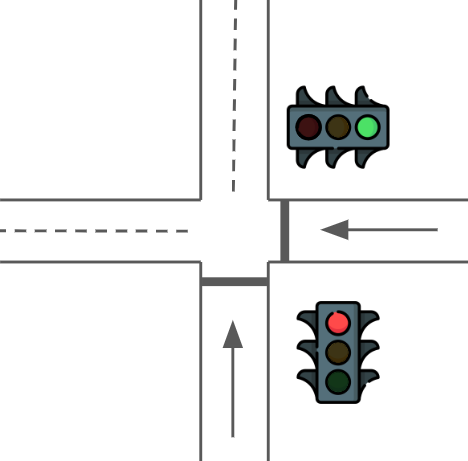
\includegraphics[width=\textwidth]{report/images/semaforossimple1.png}
        \caption{Fase 1.}
        \label{fig:semaforo-simple-1}
    \end{subfigure}
    \hfill
    \begin{subfigure}[t]{0.32\textwidth}
        \centering
        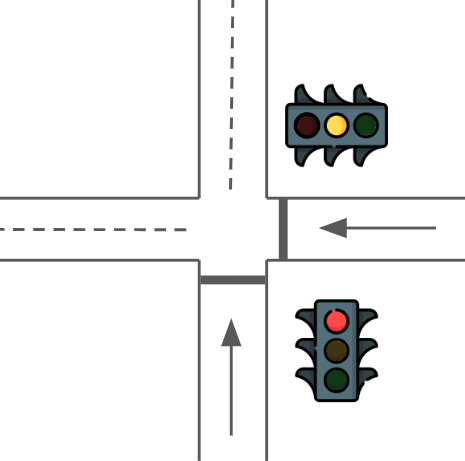
\includegraphics[width=\textwidth]{report/images/semaforossimple2.png}
        \caption{Fase 2.}
        \label{fig:semaforo-simple-2}
    \end{subfigure}
    \hfill
    \begin{subfigure}[t]{0.32\textwidth}
        \centering
        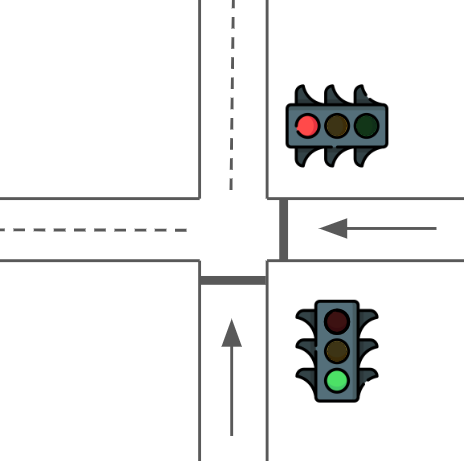
\includegraphics[width=\textwidth]{report/images/semaforossimple3.png}
        \caption{Fase 3.}
        \label{fig:semaforo-simple-3}
    \end{subfigure}
    \caption{Cambio de fases en una intersección.}
    \label{fig:semaforo-simple}
\end{figure}

Cada una de las fases de esta intersección tienen una duración asignada. Por ejemplo, podríamos asignar una duración a la fase 1 (figura~\ref{fig:semaforo-simple-1}) podría de 30 segundos, mientras que la 2 (figura~\ref{fig:semaforo-simple-2}) duraría 4 segundos (dado que es una fase que contiene un semáforo en ámbar), y finalmente la fase 3 duraría 45 segundos. Este conjunto de duraciones es una posible solución a nuestro problema, que al final lo que busca es asignar las duraciones a las fases de los semáforos de modo que permitan circular al tráfico de la manera más eficiente, y es con lo que lidiaría el algoritmo evolutivo. Así es, pues, como se representa el fenotipo.

\textbf{El genotipo}, por otro lado, es la codificación de nuestra solución, es la manera en que representamos los individuos de modo que el algoritmo evolutivo pueda trabajar con ellos. Para el caso en cuestión, el fenotipo mostrado por la figura~\ref{fig:semaforo-simple} lo representaríamos por un \textit{array} de valores que se corresponderían con las duraciones de dichas fases. Por ejemplo: \texttt{[30, 4, 45]}. Suponiendo que contásemos con varias intersecciones, cada una de ellas compuesta de varios semáforos, y cada uno de estos compuestos de varias fases con sus respectivas duraciones, simplemente se añadirían al \textit{array} dichas duraciones como valores numéricos igual que antes: \texttt{[30, 4, 45, 20, 55, 4, 80, 22, 47, 4, ...]}.

Vale la pena mencionar que, además de lidiar con duraciones de fases, el \textit{array} también contendrá valores numéricos en representación de los retardos de las intersecciones (véase la figura~\ref{fig:genotipo}). Estos retardos son los que se emplean para sincronizar varias intersecciones con semáforos de modo que se produzcan las denominadas \textit{oleadas de verde}~\cite{segredo_optimising_2019}.


\begin{figure}[ht]
    \centering
    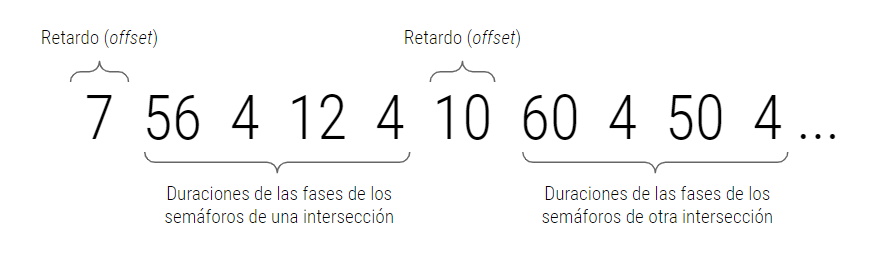
\includegraphics[width=\textwidth]{report/images/genotipo.png}
    \caption{Ejemplo de genotipo.}
    \label{fig:genotipo}
\end{figure}

\section{Aplicación del algoritmo y estudio estadístico sobre los parámetros óptimos de ejecución}

Con el objetivo de mejorar el funcionamiento del algoritmo y saber que se están empleando los parámetros adecuados de configuración para obtener los mejores resultados, se ha realizado un estudio estadístico que alterna distintos parámetros del algoritmo evolutivo.

Este estudio se ha realizado por separado para cada una de las instancias detalladas en la sección~\ref{subsec:instancias}, dado que son las únicas que requieren el empleo del algoritmo.

\subsection{Parámetros de configuración}

Las variables tenidas en cuenta para el estudio estadístico han sido dos:

\textbf{Cruce} \textit{(Crossover)}. A la hora de evaluar el cruce entre genotipos, se han valorado dos opciones: \texttt{OnePointCrossover} y \texttt{UniformCrossover}.

\begin{itemize}
    \item \texttt{OnePointCrossover} intercambia un único punto (situado en la misma posición) de ambos genotipos. Por ejemplo: supongamos que manejamos dos genotipos distintos, los cuales podemos representar en binario: 0000 y 1111. \texttt{OnePointCrossover} se limitará a seleccionar una posición aleatoria, la cual será la misma para ambos genotipos, y dividirá el genotipo en dos <<secciones>> distintas, partidas por esa posición mencionada. A continuación, intercambiará entre entre ambos genotipos las mitades de uno de los lados. En el caso del genotipo anterior, si la posición seleccionada es la correspondiente al tercer elemento de izquierda a derecha, el resultado después del cruce sería 0011 y 1100 para el primer y el segundo genotipo, respectivamente.
    \item \texttt{UniformCrossover}, por otro lado, intercambia elementos individuales entre sí, cuyas posiciones son seleccionadas aleatoriamente en función de un umbral que determina la probabilidad de que se produzca dicho intercambio. Tomando los genotipos anteriores, 0000 y 1111, y un umbral de 0.50, un posible resultado de aplicar el cruce podría ser 1001 y 0110 para el primer y segundo genotipo, respectivamente. Véase como, en este ejemplo ideal, un 50 \% de los puntos han sido intercambiados entre sí, en consonancia con el umbral marcado.
\end{itemize}


\textbf{Población} \textit{(Population)}. La población determina la cantidad de individuos que son procesados durante una generación. En particular, se han seleccionado dos valores: 10 y 50.

Junto con las variables mencionados, el algoritmo evolutivo se ha ejecutado, para el estudio estadístico, con los siguientes parámetros:

\begin{itemize}
    \item Generaciones: 50. 
    \item Generación aleatoria de valores para los individuos: uniforme entre 4 y 120 (sin embargo, devolverá 4 cuando el individuo contenga alguna duración de un semáforo en fase ámbar).
    \item Selección: \texttt{RouletteWheel}.
    \item Mutación: \texttt{RandomResseting}, con $r = 1 / g$, donde $r$ es el ratio de mutación y $g$ la cantidad de genes. Para la instancia actual, $r \approx 0.01$.
    \item Condición de terminación: por generaciones.
\end{itemize}

Con respecto a la simulación, se han tenido en cuenta los siguientes parámetros:

\begin{itemize}
    \item Duración de la simulación: 1800 segundos (30 minutos, tramo 8:00-8:30).
    \item Tiempo para teletrasporte: 120 segundos.
\end{itemize}


\subsection{Proceso del estudio estadístico}

Este estudio se centra en analizar si existe algún tipo de diferencia estadística en los resultados de emplear unos parámetros u otros, de modo que al final se empleasen los que mejor resultado devolvieran. Para este estudio se han tenido en cuenta dos parámetros: cruce y tamaño de población, para cada una de las  cuatro instancias citadas en la sección~\ref{subsec:instancias}.

Contando con que tenemos 4 instancias que simular, y dado que para cada una de ellas hay 2 variables, cada una de ellas con 2 posibles valores, en total han de realizarse 16 ejecuciones en total: la primera instancia con una población de 10 individuos y usando un cruce tipo \texttt{OnePointCrossover}, la misma instancia pero variando el cruce, luego variando la población, y luego ambos; y de igual modo para el resto de las instancias.

Además, en aras de unos resultados más robustos, cada una de las 16 configuraciones se ha ejecutado 10 veces con semillas distintas, para evitar que pudiera derivarse algún tipo de sesgo e introducir aleatoriedad en la simulación, algo que sucede en la vida real puesto que no hay dos días en que todos los vehículos y peatones realicen exactamente la misma ruta en el mismo momento. En cada una de esas ejecuciones también han de contarse las generaciones y los individuos de cada una de estas, puesto que cada individuo obtiene su valor de fitness a partir de los resultados de la simulación. Así pues, dado que todas las ejecuciones han tenido como parámetro 50 generaciones, y dado que la mitad de las 16 configuraciones empleaban 10 individuos y la otra mitad 50, el cúmulo de simulaciones realizadas se eleva a las 240.000.

$$
S = \sum_{1}^{i} C_i * G * I_i * E
$$

donde $S$ es el número de simulaciones realizadas, $i$ es la cantidad de valores seleccionados para la cantidad de individuos (en este caso, 10 y 50, por lo que $i=2$), $C_i$ equivale a la cantidad de configuraciones que empleaban $I_i$ individuos (de las 16 configuraciones, la mitad empleaba 10 y la otra 50, por lo que $A_1 = A_2 = 8$), $G$ es la cantidad de generaciones (50, igual en todos los casos) y $E$ la de ejecuciones (10, es un valor fijo). Sentado lo anterior:

$$
S = (8*50*10*10) + (8*50*50*10) = 240.000
$$

Dado que cada una de las ejecuciones dura aproximadamente 30 segundos, el tiempo estimado (suponiendo que se ejecutasen secuencialmente) para completar el estudio es de aproximadamente 2000 horas (83 días). Por suerte, se ha contado con Bólido para llevar a cabo el estudio, el cual cuenta con 50 núcleos que han reducido el tiempo de cómputo a dos días.

Para determinar qué conjunto de parámetros es mejor para una instancia particular, el algoritmo ejecutado para llevar a cabo el estudio estadístico evalúa dos posibles conjuntos entre sí para determinar de ellos cuál es mejor. Como hemos visto antes, hay 2 parámetros (recordemos, cruce y cantidad de individuos por generación; llamémosles $P_{1x}$ y $P_{2x}$) con 2 posibles valores cada uno, lo cual representamos con la $x$. Así pues, podríamos contar con que tenemos $P_{11}$, $P_{12}$, $P_{21}$ y $P_{22}$ conjuntos de parámetros que estamos valorando para cada instancia; dónde, por ejemplo, $P_{11}$ equivale a \texttt{OnePointCrossover} y 10 individuos. 

Bien, el algoritmo evaluará los resultados que ofrece emplear el conjunto $P_{11}$ contra $P_{12}$, luego contra $P_{21}$; y así sucesivamente. Cuando haya terminado de evaluar dicho conjunto, continuará evaluando el siguiente ($P_{12}$) contra el resto salvo el primero, y así hasta que todas las combinaciones (sin repeticiones) de parejas posibles hayan sido comparadas entre sí.

Para determinar cuándo hay una diferencia estadística entre un conjunto u otro el algoritmo recibe como entrada dos vectores de valores (uno por conjunto de parámetros) a los cuales se les aplican varios tests estadísticos y que denominaremos $\vec{Q}_x$.

Cada vector contiene 10 valores, uno por cada ejecución (mencionada en párrafos anteriores). Cada una de las ejecuciones del algoritmo se ha llevado a cabo con 50 generaciones. Así pues, para determinar el valor de un elemento del vector, se ha seleccionado el valor de fitness del mejor individuo de cada una de las 50 generaciones y se ha realizado la media. Así pues, en cada vector tenemos las medias del fitness de los mejores individuos por generación de cada ejecución.

Luego, una vez que contamos con ambos vectores, se les aplica el test de Shapiro para determinar el p-value de cada conjunto. Si algún p-value es menor a 0.05, se pasa directamente al test de Kruskal Wallis; si no, ambos p-value son mayores a 0.05, por lo que se cumple el test de normalidad y se ejecuta el test de Levene para analizar las varianzas entre ambos conjuntos. Si dicho test devuelve un resultado mayor a 0.05, las varianzas no presentan una diferencia significativa y por tanto el p-value final se calcula con el test de Anova. En caso de que las varianzas sí presenten una diferencia significativa, dicho p-value se calcula con el test de Welch.

Una vez que hemos pasado la serie de tests anteriores, tendremos un p-value final. Si es superior a 0.05, se asume que no hay diferencia entre aplicar uno u otro conjunto puesto que ambos ofrecerán el mismo resultado; pero si es inferior a 0.05 existe una diferencia estadística entre ambos conjuntos de parámetros y, para determinar cual es mejor, se selecciona el que tenga mayor mediana calculada a partir de los elementos del vector $\vec{Q}_x$ del conjunto.

Los resultados de este estudio se comentarán en su respectiva sección en el capítulo siguiente.